% !TeX root = ../thuthesis-example.tex

\chapter{Sequence-based Method}

\section{Introduction}

Current models for predicting the Michaelis constant primarily utilize sequence-based approaches, each employing distinct strategies to model enzyme-substrate interactions. Some models, such as \citeauthor{km1}, rely on simple embeddings to represent protein sequences, highlighting the potential of basic representational techniques. Conversely, models like ENKIE utilize Bayesian Multilevel Models (BMMs) to incorporate enzyme properties hierarchically, though they do not directly utilize the protein sequences. \cite{enkie} Among these, ProSmith stands out by pre-training large, enzyme-specific protein models and utilizing embeddings from comprehensive protein models, showcasing advanced capabilities in capturing complex interactions. \cite{prosmith}

In this context, we introduce SeqKm, a deep learning model that leverages the extensive knowledge encoded in pre-existing large protein models without the necessity for additional pre-training. This approach not only facilitates quicker training and prediction times but also aims to enhance model performance by utilizing the inherent protein knowledge present in these large models.

Our analysis focuses on comparing SeqKm to the current state-of-the-art models in this field. Although SeqKm does not surpass ProSmith in overall performance, it achieves comparable results on a newly curated test set. This equivalence in performance suggests SeqKm's superior generalization capability and presents promising results for ensemble methods in the accurate prediction of Michaelis constants.

\section{Methods}

We now describe our input representation, model achitecture, training details, and results. 
Figure \ref{fig:seqkm} provides an overview of our method.

\begin{figure}
  \centering
  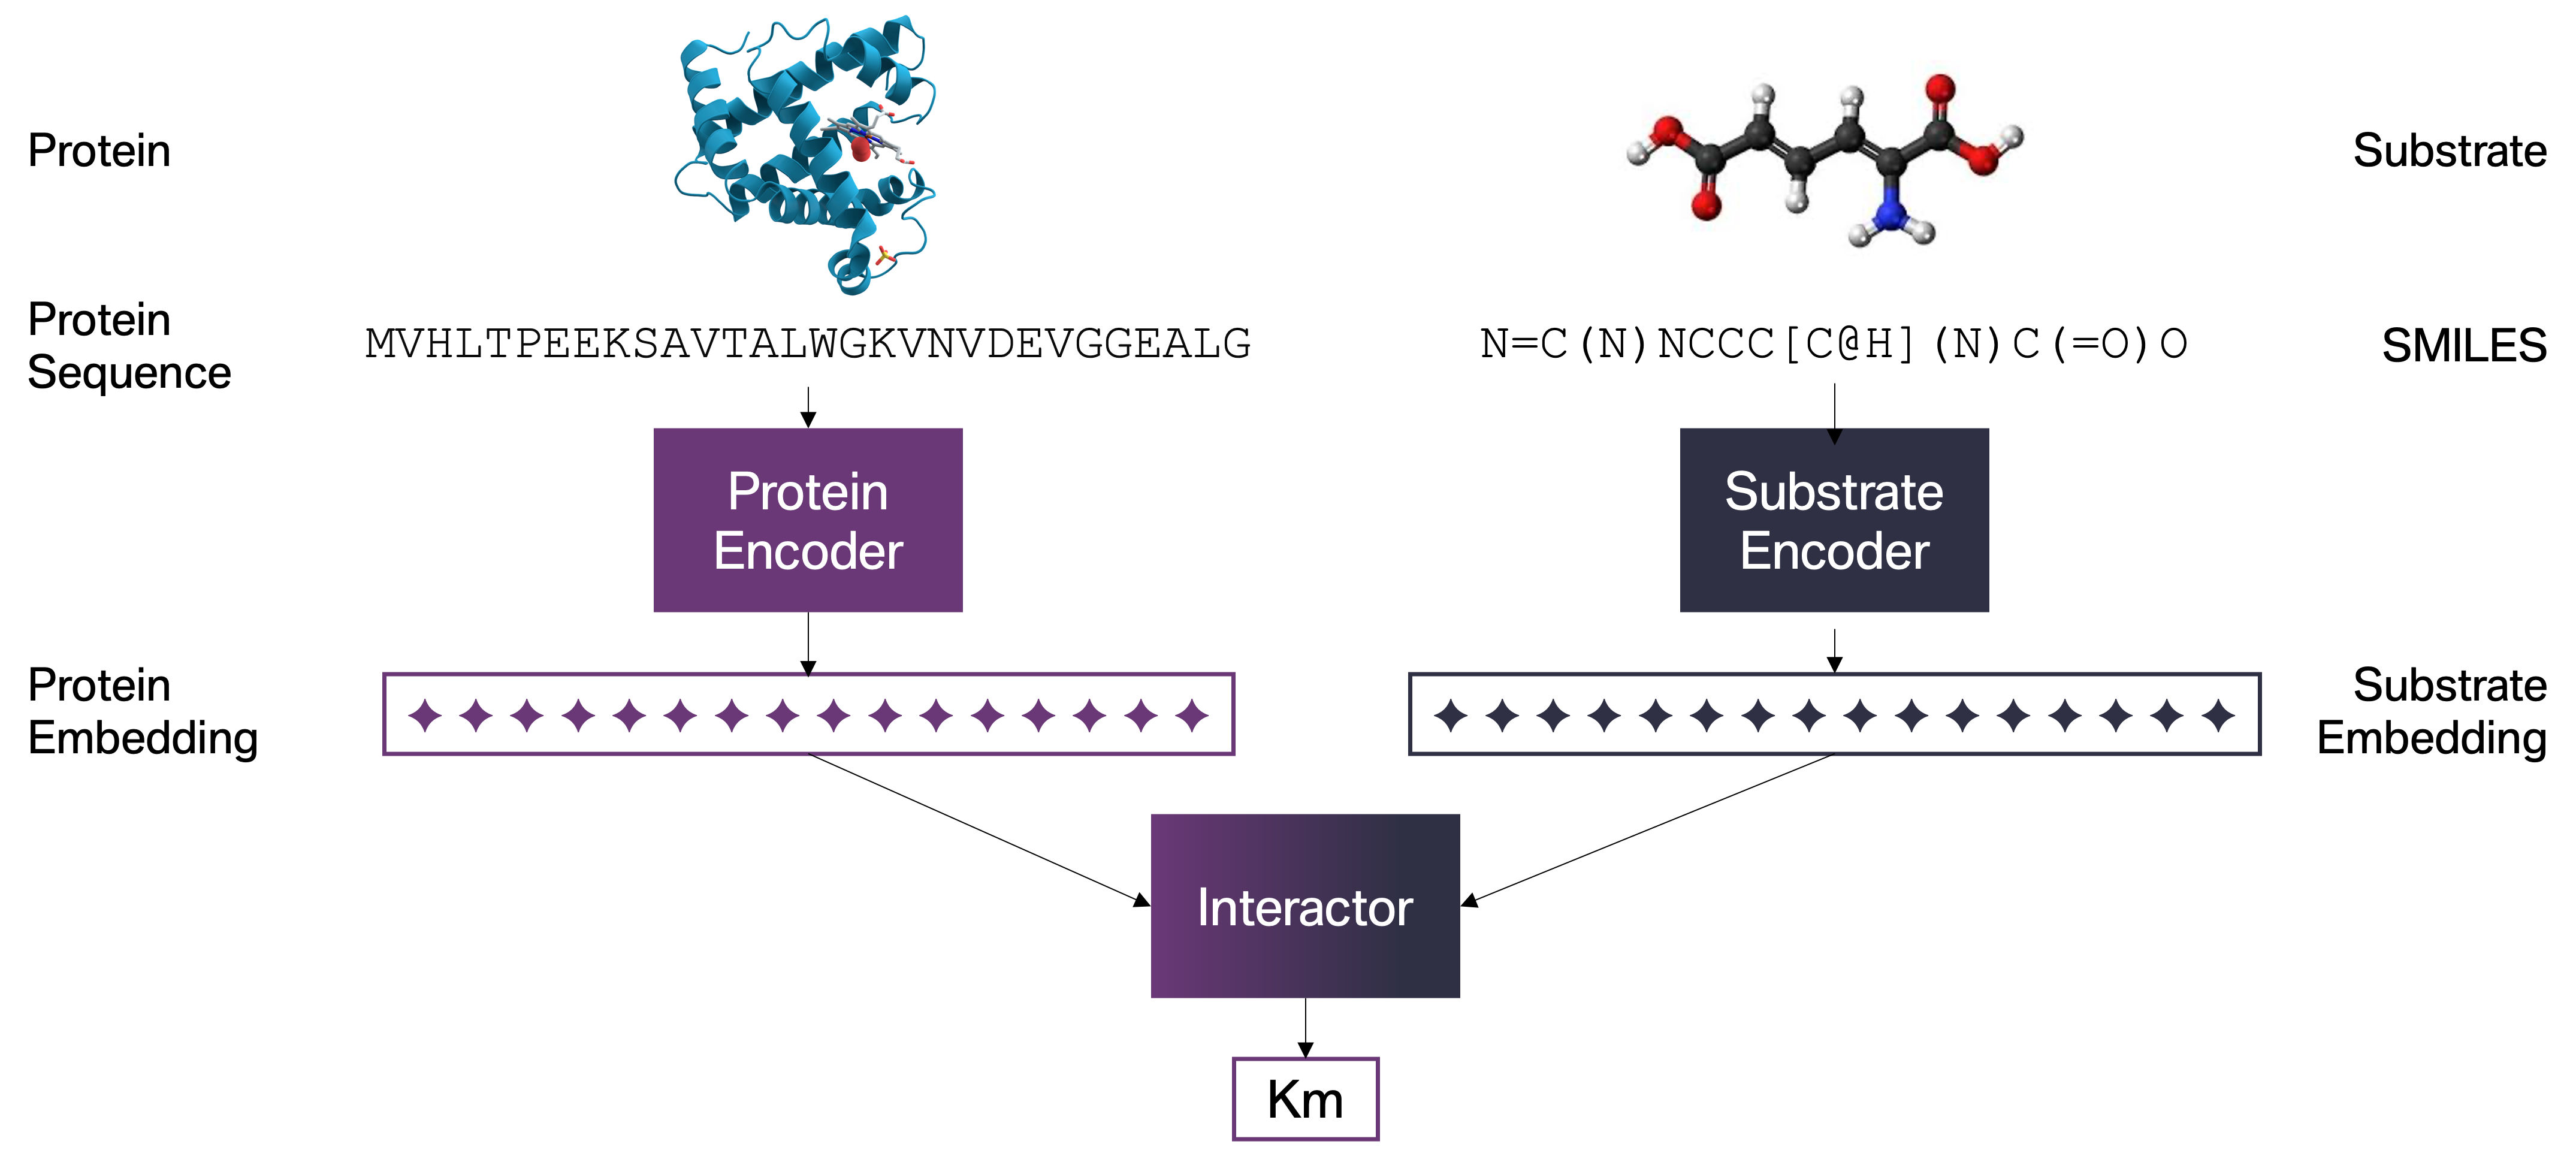
\includegraphics[width=1\linewidth]{2-sequence_architecture.png}
  \caption{Overview of SeqKm}
  \label{fig:seqkm}
\end{figure}

\subsection{Input representation}

We are given a protein sequence of length $n$ $P=a_1a_2a_3...a_n$ where $a_i$ represents the amino acid
at position $i\in\{1,..,n\}$ and each $a_i$ is an element from the set of 20 standards amino acids to
which we added an unknown amino acid $X$: $A=\{A,C,D,E,F,G,H,I,K,L,M,N,P,Q,R,S,T,V,W,Y,X\}$.

As a string cannot directly be processed by a deep learning model, a tokenization step is necessary. As
the ProtT5-XL model will be used, its tokenizer will also be used to prepare the protein sequences \cite{prottrans}.
The ProtT5-XL tokenizer is made on a vocabulary containing all the 20 amino acids but also other unsure or less
common amino acids such as B that refers to asparagine (N) and aspartic acid (D) when the specific
amino acid cannot be determined. It also has a padding token <pad>, an unknown token <unk>, a end
token </s> to indicate the end of the sequence, and some additional tokens for special cases.

Hence, all protein sequences are first truncated or padded to length 1023 and then tokenized to have inputs of
length 1024: 1023 amino acids or pad tokens <pad> and the end token </s>. This input can be used for downstream
applications.

We are also given a substrate string in its SMILES form. This can be defined as a $S=c_1c_2c_3...c_n$
where $c_i$ represents the chemical symbol for the atom at position $i\in\{1,...,n\}$ in the SMILES
sequence, or a symbol representing a bond or branching in the molecule.

Similarly, it first needs to be processed in a format that can be processed by a statistical model. To do so,
we use the Morgan Fingerprints that represent a small molecule in a way that can easily be used for computational
tasks such as ours. We selected a vector size of 1024 to be consistent with the size of the protein sequence. We
also choose to use a radius size of 1, indicating that each atom of the molecule is updated only once based on its
immediate neighbors.

We know have two inputs that can be processed by a machine learning model.

\subsection{Model Architecture}

Our model is composed of three modules: a protein encoder that encode the protein, a substrate encoder that
encode the substrate, and an interactor that makes the encoded protein and the encoded substrate interact.

The protein encoder is composed of the ProtT5-XL model to which we relaxed the 2 last layers during the training.
Relaxing is a selective fine-tuning strategy that allows to slightly adjust certains weights of a pretrained model 
to better perfom on our specific task. The decision of relaxing only the 2 last layers of the model is based on
the assumption that these layers contain the most task-specific information, while ealiest layers usually capture
universal features. This not only render the training faster are only a few weights need to be updated during the
fine-tuning process while still making the model adapted to our specific task.

The protein encoder output a matrix of size $1024\times 1024$ with the first one being the length of the sequence,
padded or not, and the second being the embedding dimension which is 1024. Technically, this mean that every
amino acid has an embedding of size 1024. Considering we are only looking for an embedding per protein sequence
and not per amino acid, we use the common technique of averaging on the amino acid dimension, leaving us with a
single vector of length 1024.

The substrate encoder for this model is simply a dummy model that does not modify the input as it was already
processed as a Morgan Fingerprints, which is already a reprensetation of the substrate as a vector of length 1024.

Finally, the interactor is a multilayer perceptron of 2 dense layers of size 256 and 128. It takes as input the
concatenated protein embedding and substrate embedding and pass it through these 2 layers to finally output a single
value, the Michaelis constant $K_m$.

\section{Training details}

We trained and validated our model using the dataset described in Section \ref{sec:dataset} as well as the new
test dataset that we currated and that contains data from 2022 to 2024. The training set contains roughly 8k
protein-substrate pairs and their $K_m$ value. The validation and testing set contains about 1k and 2k pairs
respectively. 

We trained our model over 300 epochs using the Adam optimizer with $\beta_1=0.9$ and $\beta_2=0.999$, and an initial
learning rate of $5\times10^{-4}$. The learning rate follows a cosine schedule, including a warmup phase of 200
steps to gradually increaser the learning rate from zero to the initial set value, ehnancing the model's convergence
stability. Training and validation batch sizes are set to 256 and 32 per device, respectively, to efficiently
utilize computational resources while maintaining an appropriate balance between speed and memory usage. 

Additionally, we leverage a cosine learning rate scheduler to adjust the learning rate dynamically, 
encouraging better fine-tuning and generalization as training progresses. To monitor the model's performance 
and ensure robustness, we log metrics every 20 steps and save the model's state every 500 steps. 
Evaluation is conducted at each step, allowing for continuous monitoring of the model's effectiveness on 
validation data. 

Finally, after looking at the best metrics for the validation test, we reverted to the saved model of the
 17th epoch. 

 \section{Results}

 Using the model and the training strategy presented above, we obtain a MSE of 0.700 and a $r^2$ of 0.493, making our model better than only one of the four models in our benchmark. We also obtain the following hot/cold results for the test set:

 \begin{table}[ht]
  \centering
  \begin{tabular}{lcccccc}
  \hline
   & \multicolumn{3}{c}{\textbf{Hot substrate}} & \multicolumn{3}{c}{\textbf{Cold substrate}} \\
   & Samples & MSE & R\(^2\) & Samples & MSE & R\(^2\) \\ \hline
  \textbf{Hot protein}  & 1192 & 0.642 & 0.485 & 64 & 0.821 & 0.449 \\
  \textbf{Cold protein} & 985 & 0.708 & 0.536 & 98 & 1.250 & -0.004 \\ \hline
  \end{tabular}
  \caption{SeqKm results on the test set}
  \label{tab:seqkm_results}
 \end{table}

 The general performance of SeqKm, when analyzed under the hot/cold framework, reveals a nuanced picture of its predictive capabilities, especially in comparison to ProSmith.

 Firstly, the overall pattern shows that SeqKm, like ProSmith, performs better with hot substrates compared to cold substrates, indicating a potential reliance on known substrate information for making accurate predictions. Specifically, the results for hot proteins and hot substrates yield an MSE of 0.642 and an correlation coefficient $r^2$ of 0.485, slightly worse than what was observed for ProSmith, where an MSE of 0.534 and an correlation coefficient $r^2$ of 0.572 were recorded under similar conditions. This suggests that SeqKm may not utilize protein information as effectively as ProSmith, or it might be more sensitive to variations in substrate quality.
 
 Moreover, the performance dip for SeqKm becomes more pronounced with cold proteins, regardless of whether the substrate is hot or cold. This is particularly evident in the drastic drop to an correlation coefficient $r^2$ of -0.004 for cold proteins and cold substrates, even lower than ProSmith's already disappointing performance in this category. Such results underscore a significant challenge for SeqKm in generalizing to completely unseen protein-substrate pairs.
 
 However, a surprising aspect of SeqKm's performance is observed in its handling of hot substrates paired with cold proteins, where it achieves an correlation coefficient $r^2$ of 0.536. This is almost as good as ProSmith's performance under similar conditions.
 
 The analysis of SeqKm, alongside with ProSmith's outcomes, raises important considerations about the current state of Michaelis constant prediction models. While SeqKm exhibits a comparative ease of training and potentially faster prediction times due to the lack of a pre-training requirement, its ability to generalize across completely novel enzyme-substrate interactions remains limited. This limitation is crucial, especially in the context of drug discovery and enzyme engineering, where the ability to accurately predict the behavior of uncharacterized proteins is invaluable.

For the new test set, we obtain a global MSE of 0.973 and correlation coefficient $r^2$ of 0.447:

\begin{table}[ht]
  \centering
  \begin{tabular}{lcccccc}
  \hline
   & \multicolumn{3}{c}{\textbf{Hot substrate}} & \multicolumn{3}{c}{\textbf{Cold substrate}} \\
   & Samples & MSE & R\(^2\) & Samples & MSE & R\(^2\) \\ \hline
  \textbf{Hot protein} & 40 & 0.787 & 0.472 & 30 & 0.851 & -0.255 \\
  \textbf{Cold protein} & 1117 & 0.884 & 0.478 & 102 & 2.066 & -0.006 \\ \hline
  \end{tabular}
  \caption{SeqKm results on the new test set}
  \label{tab:updated_summary_performance}
\end{table}

For the general metrics, we obtain results that are closer to ProSmith for the new test set, even though still below. We notice that whereas ProSmith had a correlation coefficent $r^2$ go from 0.563 to 0.467 (20\% drop) between the test set and the new test set. While are results are inferior, from 0.493 to 0.447 (10\%), the drop in percentage is twice as small, indicating that our model is more robust to new samples.

Furthermore, we notice that similarly to ProSmith, the results are better for cold proteins and hot substrates than for hot proteins and substrates, which indicates that our sequence-based model seems to deal with the same problems than ProSmith, in additional to smaller results in general.

We also have the same pattern for the hot proteins and cold substrates. While the MSE is relatively small compared to the other groups, the correlation coefficient $r^2$ is negative and even larger than ProSmith's. This indicates that our model cannot properly predict the Michaelis constant when the protein is known but the substrate is unknown, and even produce values that are inversely proportional, which would be a huge problem for wet-lab experiments.

Finally, we also obtain poor performance for the cold proteins and cold substrates group, indicating once again that our model, similarly to ProSmith, is incapable of generalizing properly to completely unseen samples.

Following the analysis of sequence-based models for Michaelis constant prediction on both the test and new test datasets, we conclude that a sequence-based approach is alone not enough to predict properly the Michaelis constant. Hence, our attention now shifts towards exploring structure-based methods. Given the limitations observed in the current models' ability to generalize across novel enzyme-substrate interactions, investigating structure-based approaches presents a promising avenue for enhancing predictive accuracy. By leveraging the detailed spatial information inherent in protein and substrate structures, we aim to ascertain whether these methods can surpass the performance of sequence-based models, potentially offering a more robust solution for predicting enzyme kinetics.